\documentclass[12pt]{article}
%importartion des différents packages
\usepackage[utf8]{inputenc}  
\usepackage[T1]{fontenc}
\usepackage{geometry}
\usepackage{graphicx}
\usepackage{hyperref}
\usepackage{bm}
\usepackage{xcolor}
\usepackage{soul}
\geometry{top=15mm, bottom=20mm, left=20mm, right=20mm} % définit les marges
\renewcommand{\baselinestretch}{1.25}  % taille de l'interligne

\title{\bf \itshape Travaux Pratiques d'Automatique \\ Synthèse Générale}
\author{Basile Masson et Alexis Kittler}

\date{Année 2022-2023}

\begin{document}

\maketitle

\section{\itshape Introduction}

Tout au long de ces quatre séances de travaux pratiques d'Automatique, nous avons utilisé la maquette n°10 dans laquelle se trouvent les deux systèmes que nous allons identifier, corriger, et enfin asservir.

\section{\itshape Réponse harmonique}

\subsection{\itshape Travail préparatoire}

    \begin{itemize} % commande pour dire qu'on démarre une liste (à puces ici)

    \item \underline{Fonction de tranfert :} Rapport entre la sortie et l'entrée d'un système. Son module représente le rapport de l'amplitude/valeur efficace de la sortie sur celle de l'entrée et son argument représente le déphasage de la sortie par rapport à l'entrée.
    \item Avant de tracer le diagramme de Bode ou de Black, il faut déterminer la nature du système (passe-bas, passe-haut, coupe-bande, passe-bande) et sa bande-passante.\\
     Une fois ceci déterminé, on génère une entrée sinusoïdale avec le GBF et on se place au début de la bande passante en modifiant la fréquence du signal avec le GBF. \\
     On affiche ensuite la sortie et l'entrée sur l'oscilloscope en simultané, et on mesure le module avec l'outil "Meas--> Amplitude" de l'oscillocope et le déphasage de la sortie par rapport à l'entrée "Meas --> Retard" à plusieurs fréquences parmi la bande passante.\\\\ En général, on mesure le plus de points quand la pulsation est à une décade de la pulsation de coupure. Il ne reste plus qu'à placer ces points, soit dans le diagramme de Bode, ou dans le diagramme de Black.
    \end{itemize}
\subsection{\itshape Travail expérimental}

\begin{itemize}
    \item \bf Système 1
\end{itemize}

\underline{Nature du système} : En prenant f très grand, on remarque que la sortie est nulle. À l'inverse, pour f = 10 Hz, la sortie est amplifiée.
Nous concluons donc que le système est de type passe-bas. Nous déterminons ensuite l'amplification statique en mesurant l'amplification pour f = 10 Hz. Nous trouvons $A \approx 1.81$.
\\De plus, nous détemrminons un ordre de grandeur de la première cassure en faisant varier la fréquence jusqu'à ce que $\frac{S}{E} = \frac{A}{\sqrt{2}}$.
En effet, lorsque l'amplification vaut $\frac{A}{\sqrt{2}}$, la pulsation correspondante est la pulsation de coupure à -3 dB. Nous trouvons comme pulsation $\omega_0 = 47  rad.s^{-1}$ ou encore $f_0 = 7,5 Hz$
\\Nous observons aussi un déphasage de -45° à cette pulsation, ce qui nous permet de conjecturer que ce système est d'ordre 1.
\\\\
Nous pouvons désormais mesurer les différents points nécessaires pour tracer le diagramme de Black : 
\\
Comme nous avons déjà un ordre de grandeur de la pulsation de coupure, nous mesurons le module et l'argument à des fréquences séparées par des intervalles plus petits lorsque ces fréquences sont proches de $\omega_0$ et on agrandit les intervalles lorsqu'on s'en éloigne.
\begin{center}
\begin{tabular}{ |p{3cm}|p{3cm}|p{3cm}|p{3cm}| }
    \hline
    \multicolumn{4}{|c|}{Points du diagramme de Black du système 1} \\
    \hline
    Fréquence $f$(Hz) & $\mid T \mid = \frac{S}{E}$ & $20 \log(\mid T \mid)$ & Déphasage $\varphi $ (°)\\
    \hline
    0.3 & 1.762 & 11.33 & -2.68 \\
    0.6 & 1.762 & 11.33 & -5.75 \\
    1.2 & 1.762 & 11.33 & -10 \\
    5 & 1.5 &  8.11 & -33.5 \\
    6 & 1.4 &  6.73 & -40.2 \\
    6.5 & 1.35 &  6.00 & -43.9   \\
    \hl{7 $= f_0$}& 1.31 & 5.40 & -44.6 $\approx 45$°\\
    7.2 & 1.31 & 5.40 & -46.5 \\
    8 & 1.22 & 3.98 & -48\\
    10 & 1.085 & 2.27 & -55\\
    11 & 1 &  0 & -56.5 \\
    15 & 0.8 &  -4.46 & -62 \\
    18 & 0.69 & -7.42 &-70 \\
    25 & 0.54 & -12.32 & -78 \\
    35 & 0.39 & -18.83 & -84 \\
    50 & 0.29 & -24.76 & -88 \\
    100 & 0.12 & -42.41 & -90 \\
    \hline
    \end{tabular}
\end{center}

Voici le diagramme de Black expérimental : 
\begin{center}
    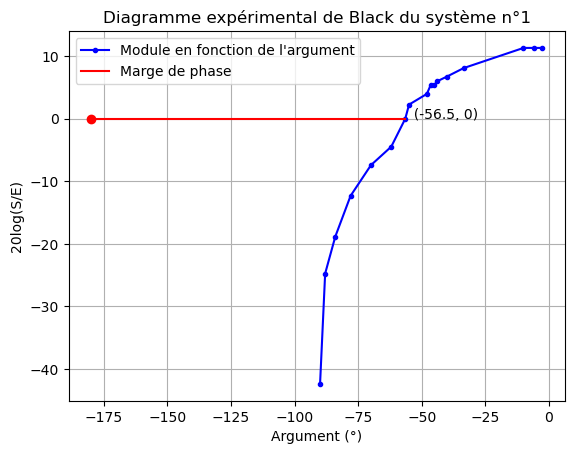
\includegraphics{TP1/Syst_1/Diagramme de Black experimental 2.1.png}
\end{center}

On remarque que ce diagramme a l'allure d'un passe-bas du $1^{er}$ ordre ($A > 0$, $\varphi \in [0^\circ,-90^\circ]$).
\\Graphiquement, la marge de phase (écart en phase entre le point à -180° et la courbe lorsque le gain est nul (sur l’axe des abscisses)) vaut $-56.5 - (-180) = 123.5^\circ$. Nous pouvions déjà déterminer la marge de phase sans le diagramme car nous avions déjà trouvé la fréquence pour laquelle $\frac{S}{E} = 1$.
\\Il suffit ensuite de mesurer le déphasage pour cette fréquence et d'y additionner 180.
\newpage


\begin{itemize}
    \item Système 2
\end{itemize}

\underline{Nature du système} : De même que pour le système 1, à fréquences très basse ($f \approx 10$Hz), l'amplitude de la sortie est amplifiée, et pour des fréquences très élevées, l'amplitude de la sortie est quasiment nulle.
\\De plus, on remarque que pour $f = 5$Hz, le quotient de l'amplitude de la sortie (S) sur celle de l'entrée est supérieur ($\frac{S}{E} = 2.26$) que pour $f = 1$Hz ($\frac{S}{E} = 2$). On interpète ceci comme étant une résonance du système autour de la fréquence 5 Hertz.
Ainsi le système 2 est un passe-bas du $2^{\grave{e}  me}$ ordre. Pour déterminer la fréquence de coupure, nous savons qu'à cette fréquence, pour un filtre passe-bas du $2^{\grave{e}me}$ ordre, le déphasage vaut $-90^\circ$ ($A = 2 > 0$). Ainsi, on trouve $f_0 \approx 7.57$Hz donc $\omega_0 \approx 47.5$Hz.

Nous pouvons désormais mesurer les différents points nécessaires pour tracer le diagramme de
Black :
Comme nous avons déjà un ordre de grandeur de la pulsation de coupure, nous mesurons le module
et l’argument à des fréquences séparées par des intervalles plus petits lorsque ces fréquences sont
proches de $\omega_0$ et on agrandit les intervalles lorsqu’on s’en éloigne.
\begin{center}
    \begin{tabular}{ |p{3cm}|p{3cm}|p{3cm}|p{3cm}| }
        \hline
        \multicolumn{4}{|c|}{Points du diagramme de Black du système 2} \\
        \hline
        Fréquence $f$(Hz) & $\mid T \mid = \frac{S}{E}$ & $20 \log(\mid T \mid)$ & Déphasage $\varphi $ (°)\\
        \hline
        0.5 & 1.95 & 13.36 & -2.51 \\
        0.6 & 1.95 & 13.36 & -4.70 \\
        1.2 & 2 & 13.86 & -9.32 \\
        2 & 2.024 &  14.10 & -15.95 \\
        3 & 2.1 &  14.84 & -25.33 \\
        4 & 2.14 &  15.22 & -36.80   \\
        5 & 2.26 & 16.31 & -49.80 \\
        6 & 2.21 & 15.86 & -65.47 \\
        7 & 2.02 & 14.06 & -82.9\\
        \hl{$7.55 = f_0$} & 1.95 & 13.36 & -90\\
        8 & 1.83 &  12.09 & -97 \\
        10 & 1.30 &  5.25 & -118.5 \\
        11.5 & 1 & 0 &-130 \\
        15 & 0.57 & -11.24 & -145 \\
        25 & 0.24 & -28.54 & -161 \\
        35 & 0.14 & -39.32 & -166 \\
        50 & 0.07 & -53.19 & -170 \\
        100 & 0.023 & -75.45 & -175 \\
        \hline
        \end{tabular}
    \end{center}

    \newpage

    Voici le diagramme de Black expérimental : 
    \begin{center}
        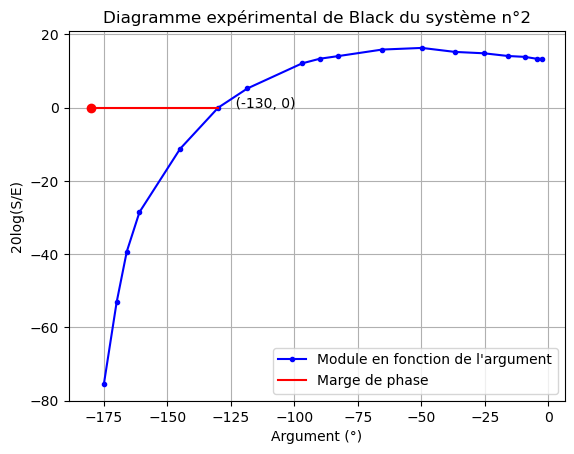
\includegraphics{TP1/Syst_2/Diagramme de Black experimental_syst2.png}
    \end{center}
    On remarque que ce diagramme a l'allure d'un passe-bas du $2^{\grave{e}me}$ ordre ($A > 0$, $\varphi \in [0^\circ,-180^\circ]$ et résonance).
    \\Graphiquement, la marge de phase vaut $-130 - (-180) = 50^\circ$.
\newpage
    \section{\itshape Réponse indicielle.Réponse Harmonique.Identification}

    Le but de cette partie est dde modéliser notre système par une fonction de transfert. Pour cela, nous allons effectuer un essai indiciel ou harmonique sur les deux systèmes.
    \subsection{\itshape Travail Préparatoire}
\begin{itemize}
    

    \item  \underline{\itshape Caractéristique statique} : Pour un système linéaire la caractéristique statique est une
    droite passant par l'origine, dans une zone linéaire la pente de cette droite est
    l'amplification statique du système.

    \item \underline{\bf \itshape Système du $1^{er}$ ordre} : Soit la fonction de transfert du $1^{er}$ ordre $F_1(p) = \frac{A}{1 + \tau p }$. Ici A représente le gain/l'amplification statique et $\tau$ représente la constante de temps (en secondes) du système.
    Pour représenter la réponse indicielle, nous savons que pour une entrée $e(t) = X_0\times\mathcal{U}(t)$, la réponse est de la forme $y(t) = AX_0(1-e^{\frac{-t}{\tau}})\mathcal{U}(t)$ avec $A$ et $\tau$ les éléments caractéristiques de $F_1(p)$.
    Ici, l'essai indiciel est modélisé avec A = 2, $X_0 = 1$ et $\tau = 0.2$s
    \begin{center}
        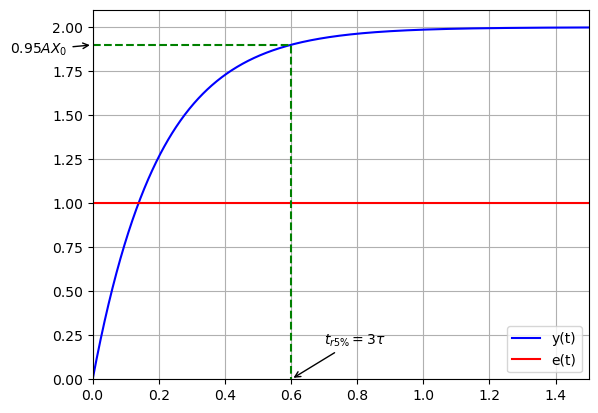
\includegraphics{TP1/Syst_1/Reponse_indicielle_prem_ordre.png}
    \end{center}
    Pour retrouver A: on fait le rapport entre l'allure de la sortie et l'allure de l'entrée en régime permanent.Pour retrouver $\tau$ : on mesure le temps de réponse à 5 $t_{r5\%}$(temps que met la sortie pour atteindre 95$\%$ 
    de sa valeur finale et y rester) et on retrouve $\tau$ grâce à la formule $t_{r5\%} = 3\tau$ (valable pour les systèmes du $1^{er}$ ordre).

    \textit{Fréquence d'observation}: pour bien observer l'allure de la sortie lorsqu'on fait un essai indiciel il faut choisir la bonne fréquence pour le signal carré d'entrée.
    \\ On doit pouvoir observer le régime transitoire et le régime permanent : si la fréquence est trop élevée on ne verra que le régime transitoire (régime permanent jamais atteint : bascule haut/bas trop
rapide) et si la fréquence est trop faible on ne verra pas le régime transitoire (il sera "écrasé" par le régime permanent). On doit donc prendre un demi-période de sorte à ce que la fréquence soit inférieure à $\frac{1}{3} \times f_0$ (car $t_{r5\%} = 3\tau$) mais pas trop pour observer le régime transitoire.
\\\\Lors d'un essai harmnonique, il suffit de mesurer la rapport de l'amplitude de la sortie sur celle de l'entrée à fréquence très basse comme ce système est un passe-bas du $1^{er}$ ordre. Pour déterminer $\tau$, on sait que à $\omega_0$, le déphasage $\varphi$ vaut $-45^\circ$. Ainsi en trouvant $\omega_0$, on trouve $\tau$ car $\omega_0 = \frac{1}{\tau}$.
\\\\\\\\
\item \underline{\bf \itshape Système du $2^{\grave{e}me}$ ordre} : Soit la fonction de transfert du $2^{\grave{e}me}$ ordre  $F_2(p) = \frac{A}{1 + 2m\frac{p}{\omega_0} + (\frac{p}{\omega_0})^2}$. 
\end{itemize}
Ici, A  représente le gain/l'amplification statique, m le coefficient d'amortissement du système et $\omega_0$ la pulsation de coupure du système.
Pour représenter la réponse indicielle, d'après le cours, nous savons que pour une entrée $e(t) = X_0\times\mathcal{U}(t)$, la réponse est de la forme  :

\begin{center}
    $y(t) = AX_0(1+A_1e^{p_1t} + A_2e^{p_2t})\mathcal{U}(t)$ 
\end{center}    
Avec $p_1$ et $p_2$ les pôles de la fonction de transfert, i.e. les racines du polynôme en p du dénominateur.
D'après le cours, si m $\ge 1$, alors $p_1 = \omega_0(-m+\sqrt{m^2-1})$ et $p_2 = \omega_0(-m-\sqrt{m^2-1})$. 
\\Et, de plus : $A_1 = \frac{\omega_0^2}{p_1(p_1-p_2)}$ et $A_2 = \frac{\omega_0^2}{p_2(p_2-p_1)}$.
Ainsi, pour A = 2, $X_0 = 1$ et $\omega_0 = 10$rad/s, on obtient le graphe suivant :
\begin{center}
    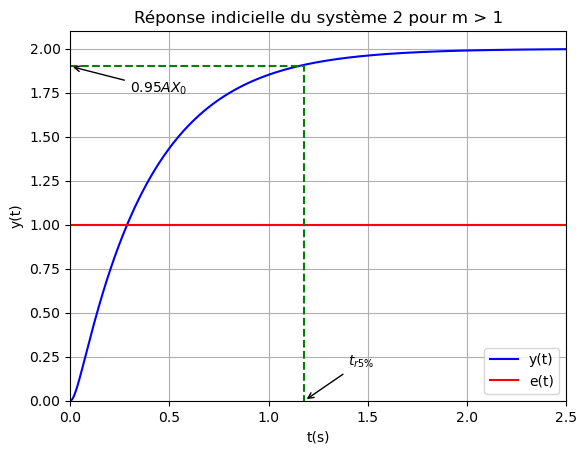
\includegraphics{TP1/Syst_2/Reponse_indicelle_m_sup_1.png}
\end{center}

On observe bien aussi la tangente nulle à l'origine, typique d'un système du deuxième ordre.

Pour $0\le m \le 1$, alors $p_1$ et $p_2$ sont complexes conjugués, i.e. $p_1 = \omega_0(-m+j\sqrt{1-m^2})$ et $p_2 = \omega_0(-m-j\sqrt{1-m^2})$.
On pose alors $p_1 = \alpha+j\beta$ et $p_2 = \alpha-j\beta$. Enfin, d'après le cours, on obtient : 
\begin{center}
    $y(t) = AX_0(1+2A_1e^{\alpha t}\cos(\beta t + \theta))\mathcal{U}(t)$
\end{center}
Avec $A_1 = |\underline{A_1}|$ car comme $p_1$ et $p_2$ sont des complexes, $\underline{A_1}$ l'est aussi.
On sait que : 
\begin{center}
 $\underline{A_1} = \frac{\omega_0^2}{\underline{p_1}(\underline{p_1} - \underline{p_2})} = \frac{\omega_0}{(\alpha + j\beta)(2j\beta)} = \frac{\omega_0}{2j\beta\alpha -2\beta^2}$
\\Il vient alors $A_1 = |\underline{A_1}| = \frac{\omega_0^2}{\sqrt{(-\beta^2)^2 + (2\beta\alpha)^2}}$
\\Après calcul, $\theta = \arg(\underline{A_1}) = \arctan(\frac{\Im(\underline{A_1})}{\Re(\underline{A_1})}) - \pi = \dots = \arctan(\frac{\alpha}{\beta^3}) - \pi$
\end{center}
On peut désormais tracer la réponse indicielle d'un système du deuxième ordre avec $m \in \left]0;1\right[$, $A = 2$, $\omega_0 = 10$rad/s, $X_0 = 1$  :
\begin{center}
    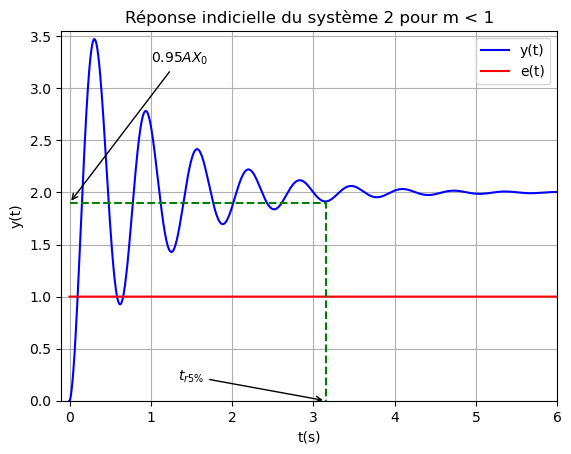
\includegraphics{TP1/Syst_2/Reponse_indicielle_m_inf_1.png}
\end{center}
\textit{Méthode de détermination des éléments caractéristiques :} On applique un signal carré en entrée, et on observe la réponse indicielle. 
\\Ensuite on mesure le $1^{er}$ dépassement (en $\%$ ) et on utilise l'abaque qui nous permet de relier le pourcentage du premier dépassement au coefficient d'amortissement.
\\Enfin, grâce à un deuxième abaque, on peut récupérer le temps de réponse réduit ($t_{r5\%}\omega_0$) avec le coefficent d'amortissement. Comme la pulsation de coupure est connue, on peut récupérer le temps de réponse à 5 $\%$.
\\\\$\underline{F_2}(j\omega_0) = \frac{A}{1 + 2m\frac{j\omega_0}{\omega_0} + (\frac{j\omega_0}{\omega_0})^2} = \frac{A}{2jm}$

\begin{itemize}
            \item $|\underline{F_2}(j\omega_0)| = \frac{A}{2m}$
            \item $\arg(\underline{F_2}(j\omega_0)) = -90^\circ$
\end{itemize}

Grâce à ces résultats, on peut extraire une méthode pour trouver $m$ et $\omega_0$ lors d'un essai harmonique: 
Faire varier la fréquence jusqu'à obtenir un déphasage de $-90^\circ$. Alors la fréquence qui correspond à ce déphasage est la fréquence de coupure $f_0$. 
\\Donc $\omega_0 = 2\pi f_0$. De plus, on sait qu'à la pulsation de coupure, l'amplification vaut $\frac{A}{2m}$. Il suffit de mesurer $\frac{S}{E}$ à cette pulsation et on peut en déduire m :
\begin{center}
    $\frac{S}{E} = \frac{A}{2m} \Leftrightarrow m = \frac{A}{2}\times \frac{1}{\frac{S}{E}}$
\end{center}

\subsection{\itshape Travail expérimental}

\subsubsection{\underline{\textit{Tracé de la caractéristique statique} }}
Comme dit dans l'énoncé de TP, nous appliquons un signal carré de très faible fréquence(500mHz) et on mesure la sortie  lorsque celle-ci atteint son régime permanent pour plusieurs valeurs d'entrée : 

\begin{itemize}
    \item \bf \large Système 1
\end{itemize}
\begin{center}
    \begin{tabular}{ |p{3cm}|p{3cm}|}

        \hline
        Amplitude d'entrée (V) & Amplitude de sortie (V)\\
        \hline
        -9.25 & -12.4 \\
        -8.25 & -12.6\\
        -7.25 & -12.4  \\
        -6.25 & -10.9 \\
        -5.25 & -9  \\
        -4.2 & -7.4  \\
        -3.15 & -5.5\\
        -2.05& -3.65  \\
        -2 & -3.65\\
        -1.55 & -2.75 \\
        0.95 & 2.72 \\
        1.45 & 3.60 \\
        2 & 3.65 \\
        2.95 & 5.5 \\
        3.95 & 7.325  \\
        4.875 & 9  \\
        5.8 & 10.9  \\
        7 & 12.8  \\
        7.87 & 12.8  \\
        9 & 12.8  \\
        
        \hline
        \end{tabular}
    \end{center}

    Et voici le tracé de la caractéristique statique :
    \begin{center}
        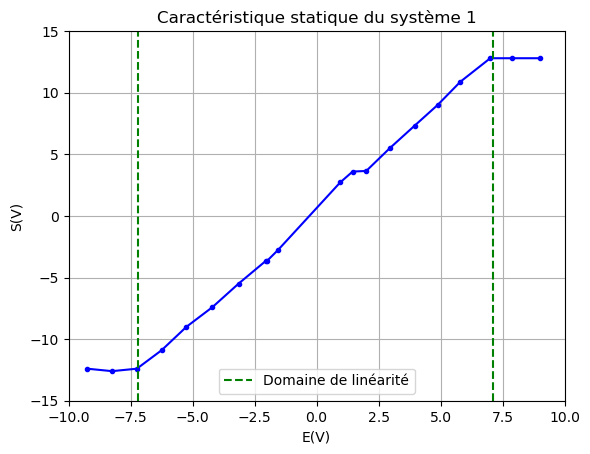
\includegraphics{TP1/Syst_1/Carac_stat_1.png}
    \end{center} 
    Grâce à cette caractéristique statique, on peut mesurer l'amplification statique, qui est la pente de \\la droite dans le domaine de linéarité ($D = \left[-7.4;7.3\right]$), qui est délimité par les pointillés en vert. On voit clairement sur le graphe que $A\approx1.8$, ce qui confirme nos résultats précédents.
    \\On peut confirmer ceci en calculant le coefficient directeur entre les points $(2.95,5.5)$ et  $(-2,-3.65)$. Ainsi $A = \frac{5.5-(-3.65)}{2.95-(-2)} = 1.84 \approx 1.8$.
   \\De plus, on peut expliquer le domaine de linéarité par le fait que les composants du système 1 (Amplificateurs opérationnels) on une tension $V_{sat}$ de saturation maximale. Si on met en entrée une tension trop élevée, l'AOP ne pourra pas l'amplifier assez vite et la sortie ne pourra pas dépasser $V_{sat}$.
\newpage
    \begin{itemize}
    \item \bf \large Système 2
\end{itemize}
\begin{center}
\begin{tabular}{ |c|c|c|c|c|c|c|c|c|c|c|c|c|}

    \hline
    Amplitude d'entrée (V) & -8.3&-6.25&-5.2&-4.2&-2&-1&1&1.9&3.75&4.8&5.75&7.93\\
    \hline
    Amplitude de sortie (V) & -12.4&-12&-10&-8&-4&-1.53&1.475&4&8&10&12&12.8\\
    \hline
    \end{tabular}
\end{center}
Et voici le tracé de la carctéristique statique : 

\begin{center}
    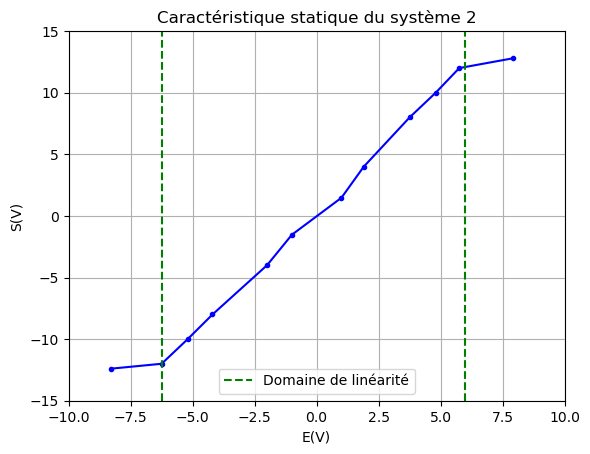
\includegraphics{TP1/Syst_2/Carac_stat_2.png}
\end{center}
Grâce à cette caractéristique statique, on peut mesurer l'amplification statique, qui est la pente de \\la droite dans le domaine de linéarité ($D = \left[-6.25;6\right]$), qui est délimité par les pointillés en vert. On voit clairement sur le graphe que $A\approx2$, ce qui confirme nos résultats précédents.
\\On peut confirmer ceci en calculant le coefficient directeur entre les points $(4.8;10)$ et  $(-6.25,-12)$. Ainsi $A = \frac{10-(-12)}{4.8-(-6.25)} = 1.99 \approx 2$. Le domaine de linéarité est expliqué par les mêmes raisons que pour le système 1.
\newpage
\subsubsection{\underline{\itshape Identification}:}
\begin{itemize}
    \item \bf \large Système 1
\end{itemize}
\textit{\underline{Essai indiciel:}} On applique un signal carré de fréquence 1Hz et d'amplitude 1V pour mesurer l'amplification statique et un signal carré de fréquence 15Hz de façon à observer à la fois le régime transitoire et le régime permanent, voici ce que l'on obtient :
\begin{center}
    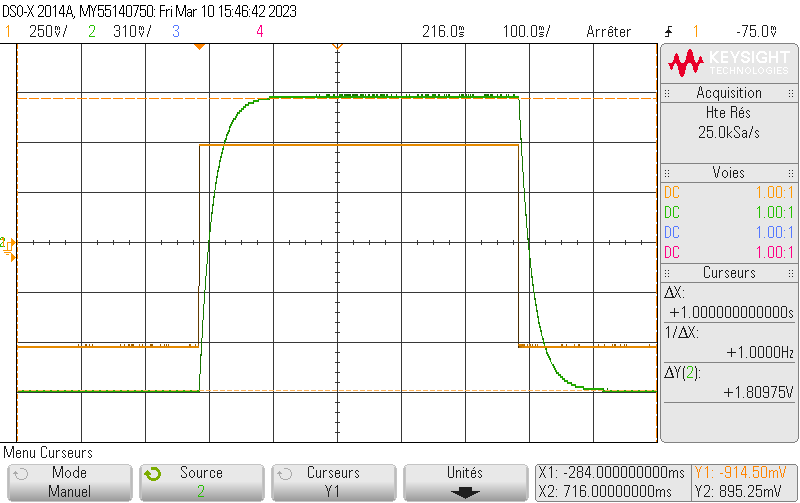
\includegraphics[width = 17 cm, height = 10cm]{TP1/Syst_1/Ampli_statique__syst_1.png}
    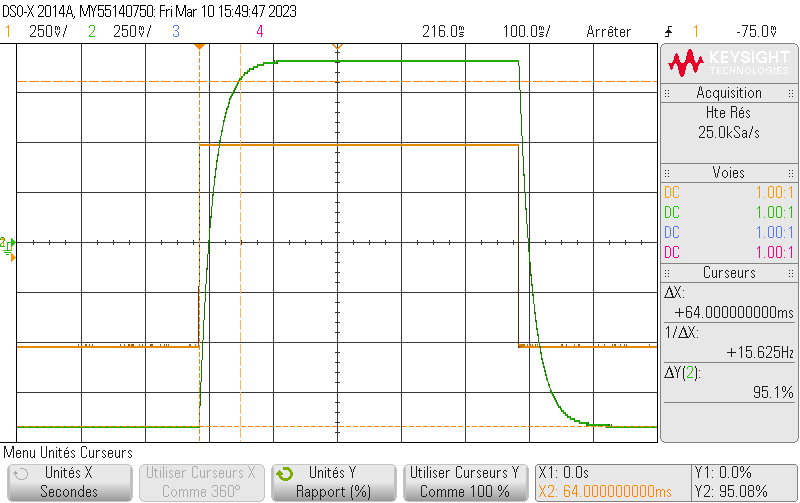
\includegraphics[width = 17 cm, height = 10cm]{TP1/Syst_1/tr5prct_syst_1_indiciel.png}
\end{center}

\begin{itemize}
    \item A : D'après le la première capture et des curseurs, avec $V_s$ en vert et $V_e$ en orange on a :
    \\$A = \frac{\Delta S}{\Delta E} = \frac{1.81}{1} = 1.81$ qui correspond à la valeur que nous avons trouvée grâce à la carctéristique statique.
    \item $\tau$ : D'après la seconde capture, le temps de réponse à 5 $\%$ est de 64ms (voir $\Delta X$ dans l'onglet "Curseurs"). 
    \\Or comme le système étudié est d'ordre 1, alors on sait aussi que :
    \\$t_{r5\%} = 3\tau \Leftrightarrow \tau = \frac{t_{r5\%}}{3} = \frac{64}{3} = 21.3$ms.
\end{itemize}
\begin{center}
Ainsi on a \fbox{$F_1(p) = \frac{1.81}{1+0.0213p}$}

\end{center}

\underline{\itshape Essai harmonique:} Similairement à la section 2.2, on retrouve A à très basse fréquence en faisant l'opération suivante : $A = \frac{\Delta S}{\Delta E} = 1.79 \approx 1.81$ qui est la même valeur qu'à l'essai indiciel.
De plus, à un déphasage $\varphi$ de $-45^\circ$, on trouve la pulsation de coupure $f_0 = 7.5$Hz donc $\omega_0 = 2\pi f_0 = 47.12$ rad/s or $\tau = \frac{1}{\omega_0} = 0.0212$s qui correspond à la valeur de $\tau$ trouvée grâce à l'essai indiciel.

\begin{itemize}
    \item \bf \large Système 2
\end{itemize}
\underline{\itshape Essai indiciel:} On applique un signal carré de fréquence 2Hz et d'amplitude 1V pour observer le régime transitoire et le régime permanent. On mesure ensuite l'amplitude du premier dépassement: 
\begin{center}
    
    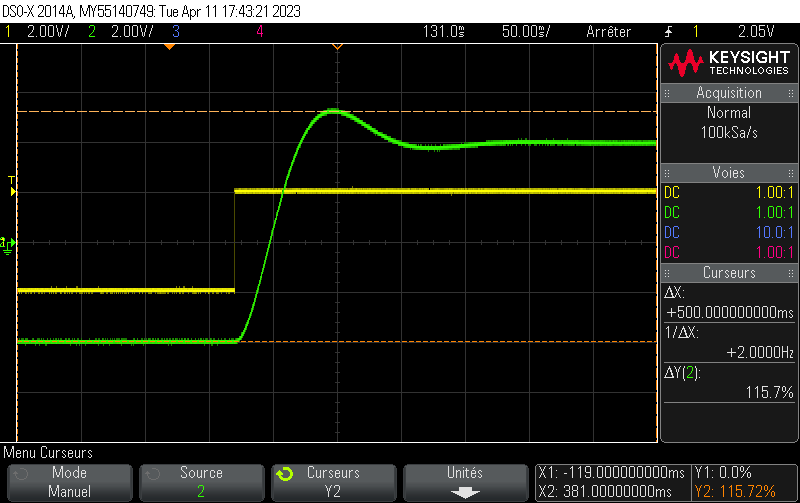
\includegraphics[width = 17cm, height = 11 cm]{TP1/Syst_2/Depassement_syst_2.png}
    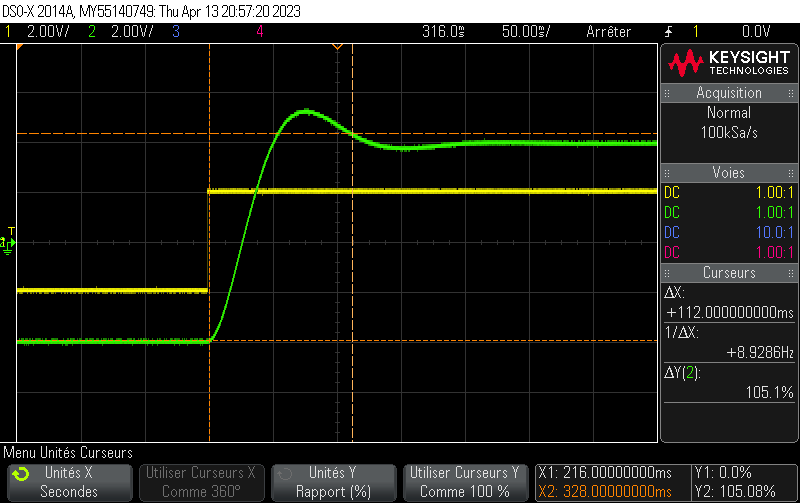
\includegraphics[width = 17cm, height = 11 cm]{TP1/Syst_2/13_04_23_tr5prct_2.png}
\end{center}
On observe donc que le premier dépassement dépasse de 15.7$\%$ la valeur finale. Il suffit ensuite d'utiliser l'abaque qui relie l'amplitude du premier dépassement au coefficient d'amortissement. Nous trouvons \fbox{$m = 0.5$}.
De plus avec le deuxième abaque et le temps de réponse à 5$\%$ (deuxième capture d'écran, $t_{r5\%} = 112$ms), on récupère le temps de réponse à 5$\%$ réduit :
\\ $t_{r5\%}\omega_0 = 5 \Leftrightarrow $ \fbox{$\omega_0 = \frac{5}{112.10^{-3}} = 44.6$ rad/s}.
\begin{center}
    Ainsi on a \fbox{$F_2(p) = \frac{2}{1 + \frac{p}{44.6} + (\frac{p}{44.6})^2}$}.

\end{center}

\underline{\itshape Essai harmonique:} Similairement à la section 2.2, on retrouve A à très basse fréquence en effectuant l'opération suivante :
\\$A = \frac{\Delta S}{\Delta E} = 2.008 \approx 2$ qui est la même valeur qu'à l'essai indiciel. De plus, à un déphasage $\varphi$ de $-90^\circ$, on trouve la pulsation de coupure $f_0 = 7.57$Hz, donc $\omega_0 = 2\pi f_0 = 47.4$ rad/s.
Mais on sait aussi qu'à $\omega_0$, $\frac{S}{E} = \frac{A}{2m}$ or $\frac{S}{E} = 2$ à $\omega_0$ donc finalement, on obtient $1 = \frac{1}{2m} \Leftrightarrow m = 0.5$ ce qui confirme nos résultats suite à l'essai indiciel.

\newpage

\section{\itshape Calcul d'un correcteur et simulations}

Nous avons désormais identifié les mesuré les éléments caractéristiques des deux systèmes. Cependant ces systèmes ne sont pas encore asservis.
\\Désormais nous allons calculer un correcteur qui permettra d'asservir nos deux systèmes.

\subsection{\itshape Travail Préparatoire}

\begin{itemize}
    \item \bf Système 1
\end{itemize}

On désire asservir le système suivant : 
\\
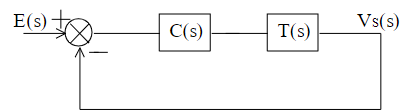
\includegraphics{TP2 Simulink/syst_a_asservir.png}

\end{document}